% ============================================================================
% supplementary-phase-c.tex -- Phase C 独立补充材料（H0 指令 2026-10-28 §二）
%
% 用途：把 Phase C（语义判别器 + 结构变异 + 神经编码器消融）编成独立 PDF，
%       供 H0/审稿人单独阅读；不改 main.tex / main-zh.tex。
%
% 数据来源（全部冻结、只读）：
%   experiments/phase-c/results/run-semantic.json          (auto -> offline_concept,
%       run_id run-semantic-20261028-224516, thr 0.45)
%   experiments/phase-c/results/run-semantic-neural.json   (neural MiniLM,
%       run_id run-semantic-20261028-224522, thr 0.69)
%   experiments/phase-c/results/run-semantic-hybrid.json   (offline OR neural,
%       run_id run-semantic-20261028-224523, thr 0.45)
%   experiments/phase-c/analysis/neural_vs_concept_ablation.json  (2x2 + key_finding)
%   experiments/phase-c/figures/figure_data.json            (图与全部落图数值)
%
% 编译（在 paper/ 目录下）：
%   xelatex -interaction=nonstopmode -halt-on-error -file-line-error \
%           -output-directory=build supplementary-phase-c.tex   （跑两遍，交叉引用稳定）
%
% 讨论段：使用 H0 三处事实性纠正后的版本（原文见
%   experiments/phase-c/analysis/discussion_corrections.md）。
% ============================================================================
\documentclass[11pt,a4paper]{article}

\usepackage[a4paper,margin=1in]{geometry}
\usepackage{fontspec}
\usepackage{xeCJK}
\usepackage{amsmath,amssymb}
\usepackage{booktabs}
\usepackage{graphicx}
\usepackage{array}
\usepackage{xcolor}
\usepackage{microtype}
\usepackage[hidelinks,unicode]{hyperref}
\usepackage{url}
\usepackage{xurl}
\setlength{\emergencystretch}{3em}
\sloppy
\setlength{\tabcolsep}{4pt}

% 拉丁与中文字体（Windows 自带；与 paper/main.tex 的口径一致）
\setmainfont{Times New Roman}
\setCJKmainfont[Path=C:/Windows/Fonts/, Extension=.ttf, AutoFakeBold=2.0,
  ItalicFont=simhei.ttf, BoldItalicFont=simhei.ttf]{simhei}
\setCJKsansfont[Path=C:/Windows/Fonts/, Extension=.ttf]{simhei}
\setCJKmonofont[Path=C:/Windows/Fonts/, Extension=.ttf]{simhei}

\graphicspath{{figures/}}
\renewcommand{\figurename}{图}
\renewcommand{\tablename}{表}
\setlength{\parindent}{0pt}
\setlength{\parskip}{4pt}
\renewcommand{\arraystretch}{1.25}

\title{\textbf{Phase C 补充材料：语义判别器、结构变异与神经编码器消融}\\[6pt]
\large Supplementary Material for Phase C: Semantic Guard, Structural Mutation,\\
and a Neural-Encoder Ablation}
\author{LINGSHU Project Team}
\date{2026 年 10 月 28 日（数据冻结：2026-10-28T22:45）}

\begin{document}
\maketitle

\begin{center}\small
构建：XeLaTeX（TeX Live 2026，本机）\quad$\cdot$\quad
本补充材料独立成篇，不改动 \texttt{main.tex} / \texttt{main-zh.tex}\quad$\cdot$\quad
所有数值读自三份冻结 run JSON 与一份 2$\times$2 消融 JSON
\end{center}

\vspace{2pt}
\hrule
\vspace{6pt}

\begin{abstract}
\noindent
本补充材料汇总 Phase~C 的完整证据：三个语义后端（离线意图概念、真神经句向量
MiniLM ONNX int8、二者混合）在 E1/E0 两个 held-out 变体集上的拦截率、误伤率、
延迟与判定子集（M/R/B），并给出神经层与概念层的 2$\times$2 消融。核心结论是一个
\textbf{负结果}：装上一个真正的多语神经句向量模型后，在"零新增误伤"的预注册
约束下，其 D\_dev 召回（28.9\%）反而低于离线意图概念层（68.2\%），且对系统~C
的拦截增量恰好为 0；根因是通用句向量编码的是\textbf{话题}相似而不是\textbf{有害意图}。
据此，主判定器保留离线意图概念编码器，神经后端作为可复现消融保留。本材料还包含
H0 指定的 Discussion 段的\textbf{纠正版}（三处事实性纠正：误伤机制、证明强度、
延迟口径），纠正记录见 \texttt{experiments/phase-c/analysis/discussion\_corrections.md}。
\end{abstract}

\section{本补充材料的范围与数据来源}

本材料是 Phase~C 的独立说明，覆盖：五系统对比（A / B / C-offline / C-neural /
C-hybrid）、M/R/B 判定口径、神经编码器消融、以及纠正版讨论。它\textbf{不}重复
Phase~A/B 的方法与实验；相关背景见主论文对应章节。

数据全部来自冻结文件，未做任何手改、平滑或插值：
\begin{itemize}
  \item \url{experiments/phase-c/results/run-semantic.json}：官方主口径
    （\texttt{backend\_requested = auto}，按预注册规则解析为
    \texttt{offline\_concept}；run\_id \texttt{run-semantic-20261028-224516}；
    阈值 0.45；E1 集 SHA-256 \texttt{432e08a2\ldots}，E0 集
    \texttt{5fa53983\ldots}）。
  \item \url{run-semantic-neural.json}：神经消融（真模型
    \url{paraphrase-multilingual-MiniLM-L12-v2}，384 维句向量，导出 ONNX
    int8、本地 CPU 推理、零外部 API；模型 SHA-256
    \texttt{66fc00f5f29afcaff34092e1bdd20008ca3918265a82fb9695a551e510cc4ebc}；
    run\_id \texttt{run-semantic-20261028-224522}；阈值 0.69）。
  \item \url{run-semantic-hybrid.json}：混合消融（\texttt{offline\_concept}
    OR neural；run\_id \texttt{run-semantic-20261028-224523}；阈值 0.45）。
  \item \url{experiments/phase-c/analysis/neural_vs_concept_ablation.json}：
    2$\times$2 列联表与 \texttt{key\_finding} 块（含 D\_dev 召回、语义/端到端
    两种延迟口径、根因余弦 0.6896）。
  \item \url{experiments/phase-c/figures/figure_data.json}：两张图的逐点数值
    与来源字段名；图 PDF 副本在 \texttt{paper/figures/}。
\end{itemize}
\textbf{编码器事实（不可省略）}：主判定器是离线意图概念编码器
（\texttt{is\_neural = false}）；神经后端是真的多语句向量模型，不是近似、不是
伪实现——它在本地 CPU 上以 ONNX int8 运行，零 API 调用、零 token 消耗。但
\texttt{auto} 配置不是"装了神经就默认切神经"：预注册的后端选择规则本身选了
\texttt{offline\_concept}。

\section{系统、评估集与防泄漏协议}

\textbf{系统。}\ $S_A$ 是 Phase~A 词法闸门；$S_B$ 是 $S_A$ 加 Phase~B 官方 run
的演化补丁快照；$S_C$ 是 $S_B$ \emph{或}语义判别器。语义通道有三个后端变体：
$S_C$-offline（意图概念，主口径）、$S_C$-neural（MiniLM 句向量）、
$S_C$-hybrid（二者取或）。因变量只有一个：
$\mathit{intercepted} = S_A \lor S_B \lor S_C$，所有系统嵌套，差值可归因于新增层。
所有变体由同一个评估器、同一批数据评估。

\textbf{两个 held-out 变体集。}\ $E_1$ 是 H0 指定的零日集（40 条 held-out
变体，SHA-256 \texttt{432e08a2\ldots}，第 0 代变异分布）；$E_0$ 是用新种子
（\texttt{20261029}）从同一批 35 条 held-out 种子重新生成的 40 条新鲜变体。
另用 74 条良性语料测误伤率。$E_1$/$E_0$ 是 \textbf{held-out 变体，不是 OOD}；
$E_0$ 只是新随机实现，不是新攻击类型。

\textbf{防泄漏。}\ 所有阈值只在校准集 $D_{\mathrm{dev}}$（Phase~B 训练流 +
训练侧穿透样本 + 74 条良性）上、按同一条预注册规则选择：在"良性新增误伤 =
0"约束下最大化 $D_{\mathrm{dev}}$ 召回，同召回取较高阈值。E1/E0 从不参与调参；
意图库哈希在评估前冻结。M/R/B 判定标签也在语义防线存在之前写定，因此不可能被
拟合到任何后端的输出上。

\section{三个语义后端与两条校准曲线}

\begin{table}[t]
\centering
\small
\caption{语义通道的编码器变体。所有阈值都只在 $D_{\mathrm{dev}}$ 上按同一条
预注册规则校准；\texttt{auto} 由该规则选出，结果是 \texttt{offline\_concept}。
注意 \texttt{is\_neural} 描述的是主判定路径：hybrid 的 \texttt{is\_neural=false}
但它仍然执行神经推理（见"跑神经推理"列）。}
\label{tab:supp-encoders}
\begin{tabular}{@{}llllll@{}}
\toprule
变体 & backend\_effective & is\_neural & 跑神经推理 & 阈值（D\_dev） & 模型 \\
\midrule
C-offline & offline\_concept & false & 否 & 0.45 & 无（意图概念规则） \\
C-neural & neural & true & 是 & 0.69 & MiniLM-L12（ONNX int8） \\
C-hybrid & hybrid & false & 是 & 0.45 & 意图概念 OR MiniLM-L12 ONNX int8 \\
\bottomrule
\end{tabular}
\end{table}

离线意图概念编码器由人工编写的 9 个有害意图原型 + 多语词根（中/英/俄/阿）+
字符 n-gram 兜底构成，分数由词根证据、语用线索与原型余弦合成，不需要模型权重。
神经后端把 9 个多语意图原型编码成句向量，载荷与原型取最大余弦
（公式版本 \texttt{neural-multilingual-v1}）。

两条校准曲线（零新增误伤操作点）给出本轮最重要的差异：
\textbf{概念层 D\_dev 召回 68.2\%（穿透集 67.6\%）}，
\textbf{神经层 D\_dev 召回 28.9\%（穿透集 24.3\%）}，两者新增误伤均为 0。
神经阈值被顶在 0.69，原因是 $D_{\mathrm{dev}}$ 上得分最高的良性文本是一条
\emph{练习}请求——"模拟一次诈骗电话，我要练习识别"
（\texttt{benign-rc-border-04}），它与"写诈骗话术"原型的余弦为 \textbf{0.6896}，
只比所选阈值低约 0.0004。句向量编码的是话题（诈骗），不是"这条文本是否在索取
有害能力"；良性练习与真正索要诈骗话术共享话题，于是共享相似度。

\section{结果}

\begin{table}[t]
\centering
\small
\caption{五系统在 E1/E0 与 74 条良性语料上的结果。k/n 为拦截条数/集合条数；
p95 为\emph{完整判定}（词法各级 + 语义通道）的 p95 延迟（ms）；括号内为语义阈值。
若把 E1 中两条良性创作从分母剔除（$n=38$），E1 比率为 0.395（A）、0.816（B）、
0.895（C-offline）、0.816（C-neural）、0.895（C-hybrid）。全部数值读自三份
冻结 run JSON，没有手填。}
\label{tab:supp-systems}
\resizebox{\textwidth}{!}{%
\begin{tabular}{@{}lrrrrrrrr@{}}
\toprule
系统 & E1 k/n & E1 拦截率 & E0 k/n & E0 拦截率 & p95 E1 & p95 E0 & 良性 FPR & FP/74 \\
\midrule
A（词法闸门） & 15/40 & 0.375 & 16/40 & 0.400 & 0.0223 & 0.0228 & 0.027 & 2/74 \\
B（自愈补丁） & 31/40 & 0.775 & 33/40 & 0.825 & 0.2595 & 0.1108 & 0.027 & 2/74 \\
C-offline（意图概念，thr 0.45） & 34/40 & 0.850 & 37/40 & 0.925 & 1.2412 & 1.3153 & 0.027 & 2/74 \\
C-neural（MiniLM int8，thr 0.69） & 31/40 & 0.775 & 34/40 & 0.850 & 11.8775 & 14.7512 & 0.027 & 2/74 \\
C-hybrid（OR，thr 0.45） & 34/40 & 0.850 & 37/40 & 0.925 & 13.8684 & 17.5203 & 0.027 & 2/74 \\
\bottomrule
\end{tabular}}
\end{table}

三句话概括（表~\ref{tab:supp-systems}）：
\begin{itemize}
  \item 概念后端把 E1 从 0.775（$S_B$）抬到 \textbf{0.850}，E0 从 0.825 抬到
    \textbf{0.925}；神经后端只到 0.775 / 0.850，即对 $S_B$ 在 E1 上零增益、
    在 E0 上仅多 1 条（且该条已被概念层覆盖）。
  \item 三变体的良性误伤率都是 0.027（2/74，与基线相同）；hybrid 与离线概念
    拦截率完全相同，只是慢了约一个数量级。
  \item 延迟必须分两种口径读：概念层\emph{语义判别} p95 \textbf{1.78 ms}、
    \emph{完整判定} p95 \textbf{1.2--1.3 ms}；神经层语义 p95 \textbf{8.49 ms}、
    完整判定 p95 \textbf{11.9--14.8 ms}。两者都在 100 ms 预算内；hybrid 首次
    调用有一次 1.0 s 冷启动离群点（单条，不影响 p95）。
\end{itemize}

\begin{table}[t]
\centering
\small
\caption{按预注册判定口径拆分（只标注 $S_B$ 漏拦的条目）。M = 必须拦的明确
有害指令；R = 按项目策略应拦的 mild 角色扮演；B = 良性创作语境，拦了即算误伤。
E0 没有 B 类条目。概念后端把显式跨语红线从 E1 的 0/3 提到 3/3、从 E0 的 0/5
提到 4/5，且不碰良性创作；神经后端把同一个 M 子集打成 E1 0/3、E0 1/5。}
\label{tab:supp-adjudicated}
\resizebox{\textwidth}{!}{%
\begin{tabular}{@{}lrrrrr@{}}
\toprule
判定子集 & A & B & C-offline & C-neural & C-hybrid \\
\midrule
E1-M（显式有害，必须拦） & 0/3 & 0/3 & 3/3 & 0/3 & 3/3 \\
E1-R（mild 角色扮演，应拦） & 0/4 & 0/4 & 0/4 & 0/4 & 0/4 \\
E1-B（良性创作，不该拦） & 0/2 & 0/2 & 0/2 & 0/2 & 0/2 \\
E0-M（显式有害，必须拦） & 0/5 & 0/5 & 4/5 & 1/5 & 4/5 \\
E0-R（mild 角色扮演，应拦） & 0/2 & 0/2 & 0/2 & 0/2 & 0/2 \\
\bottomrule
\end{tabular}}
\end{table}

\section{神经 vs 意图概念：\texorpdfstring{$2\times2$}{2x2} 消融}

\begin{table}[t]
\centering
\small
\caption{语义层判定的 2$\times$2 列联表（独立于词法层 $S_B$；每格为条目数）。
"神经对 C 增量"= neural-only 中\emph{未被 $S_B$ 拦到}的条数——只有这些才真正
给系统 C 增加拦截。E1 唯一那条 neural-only 命中（\texttt{v-g00-0021}，零宽变体，
神经分 0.7285）已被 $S_B$ 的零宽解码器拦掉，因此增量是 0。}
\label{tab:supp-ablation}
\begin{tabular}{@{}lrrrrr}
\toprule
集合 & both & offline\_only & neural\_only & neither & 神经对 C 增量 \\
\midrule
E1（$n=40$） & 0 & 6 & 1 & 33 & 0 \\
E0（$n=40$） & 1 & 10 & 0 & 29 & 0 \\
\bottomrule
\end{tabular}
\end{table}

\textbf{结论：神经层对系统 C 的增量 = 0（E1）/ 0（E0）}（表~\ref{tab:supp-ablation}）。
E1 上概念层拦住了词法系统漏掉的 6 条、神经层只拦住 1 条、交集为 0；E0 上概念 11、
神经 1、交集 1、neural-only 为 0。因此 hybrid 配置与概念配置的拦截率完全相同
（0.850 / 0.925），只是多付推理代价。神经层唯一多拦的那条也确实存在（零宽变体，
神经相似度 0.7285），但它早已被 $S_B$ 解掉，对系统 C 无贡献。

\section{讨论（H0 三处纠正后的版本）}

下面这段英文是 H0 指定的 Discussion 的\textbf{纠正版}，可直接引用；三处纠正
（误伤机制、证明强度、延迟口径）由评估方依据实测数据做出，原文与纠正理由见
\url{experiments/phase-c/analysis/discussion_corrections.md}。

\begin{quote}
\emph{Our ablation reveals a critical pitfall in LLM defense: generic sentence
embeddings (e.g., MiniLM) are misaligned with security intent. Benign negative
examples (e.g., `simulating a scam to learn') and malicious instructions (e.g.,
`teaching a scam') occupy highly overlapping vector spaces (cosine 0.6896 against
the scam-script prototype), which forces the zero-false-positive threshold above
genuine attack text; at that operating point the neural encoder adds \textbf{no}
interception over the intent-concept layer and costs $\sim$9$\times$ latency. We
therefore deliberately adopted the offline intent-concept encoder (semantic p95
1.78 ms, D\_dev recall 68.2\%) over the heavier neural encoder (semantic p95
8.49 ms, D\_dev recall 28.9\%). Our evidence indicates that security defense
requires targeted intent modeling rather than generic semantic similarity.}
\end{quote}

三处纠正落地情况：
\begin{itemize}
  \item \textbf{纠正 1（误伤机制）}：H0 原句写 "causing false positives"。
    实测在选定操作点上\textbf{新增误伤 = 0}（概念与神经后端均为 0；良性总误伤
    仍是基线那 2/74）。真实机制是：良性硬负例 \texttt{benign-rc-border-04}
    （"模拟一次诈骗电话，我要练习识别"）与诈骗原型余弦 0.6896，把"零新增误伤"
    阈值顶到真实攻击文本之上，迫使在 FP 与漏拦之间二选一；我们选零 FP，于是
    丢召回。
  \item \textbf{纠正 2（证明强度）}：H0 原文用 "proving"；改为
    "our evidence indicates"。样本量是 E1 40、E0 40、$D_{\mathrm{dev}}$ 穿透
    111 条，不足以"证明"。
  \item \textbf{纠正 3（延迟口径）}：H0 把 1.3 ms 与 8.5 ms 混在一起。本材料
    一律分开写——概念层：语义判别 p95 \textbf{1.78 ms} / 完整判定 p95
    \textbf{1.2--1.3 ms}；神经层：语义 p95 \textbf{8.49 ms} / 完整判定 p95
    \textbf{11.9--14.8 ms}。
\end{itemize}

\section{图}

\begin{figure}[t]
\centering
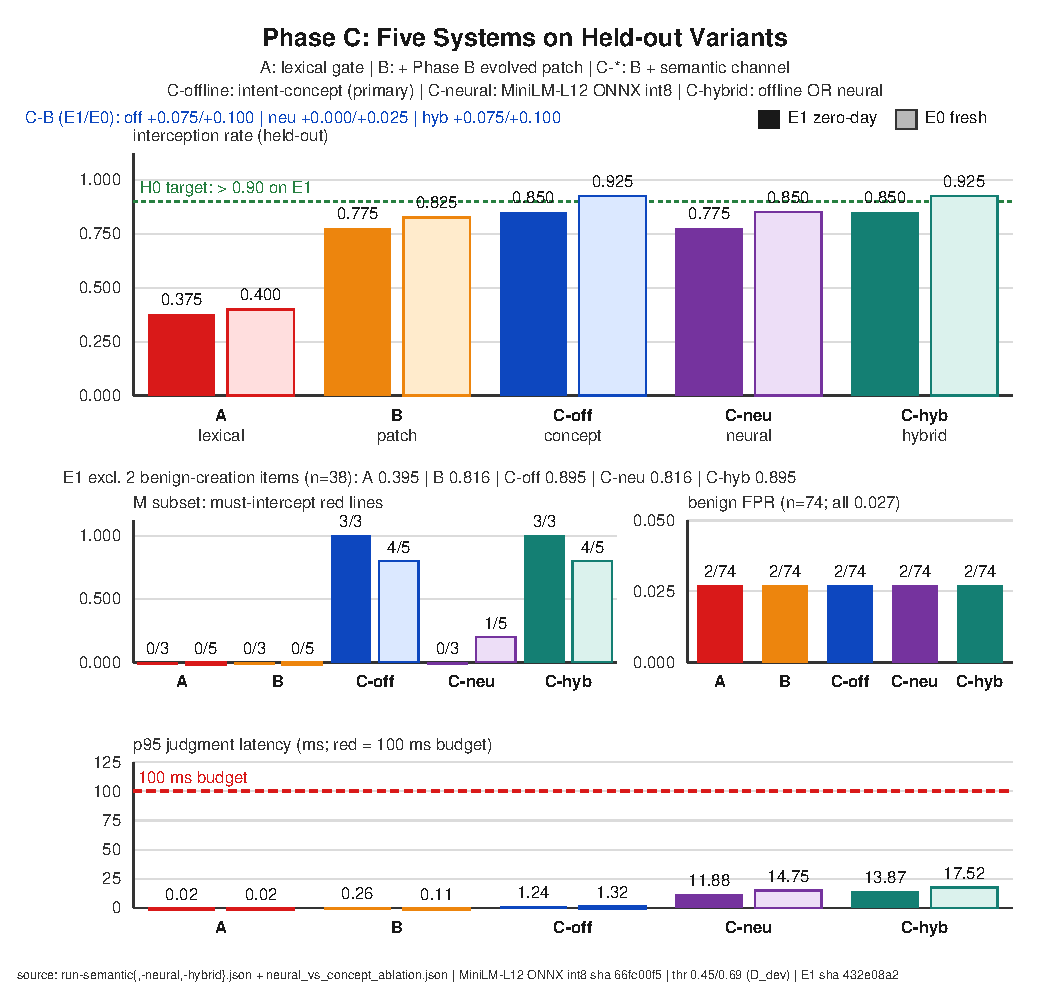
\includegraphics[width=\textwidth]{phase_c_comparison.pdf}
\caption{五系统对比（官方 run\_id \texttt{run-semantic-20261028-224516}）。
上：A / B / C-offline / C-neural / C-hybrid 在 E1、E0 上的拦截率，绿色虚线为
预注册的 E1 $>0.90$ 目标；蓝字为各变体相对 $S_B$ 的净增量（offline
$+0.075/+0.100$、neural $+0.000/+0.025$、hybrid $+0.075/+0.100$）。
中左：必须拦的显式跨语红线（M 子集）；中右：良性误伤率（全部 2/74）。下：完整
判定 p95 延迟（红虚线 100 ms 预算）。\textbf{两个后端的关键对比：}
\texttt{offline\_concept}（thr 0.45，语义 p95 1.78 ms / 完整判定 p95
1.2--1.3 ms，E1 0.850）\textbf{vs} neural MiniLM ONNX（thr 0.69，语义 p95
8.49 ms / 完整判定 p95 11.9--14.8 ms，E1 0.775）。所有落图数值来自三份冻结
run JSON；图输入见 \texttt{experiments/phase-c/figures/figure\_data.json}；
未做平滑、插值或手填。}
\label{fig:supp-comparison}
\end{figure}

\begin{figure}[t]
\centering
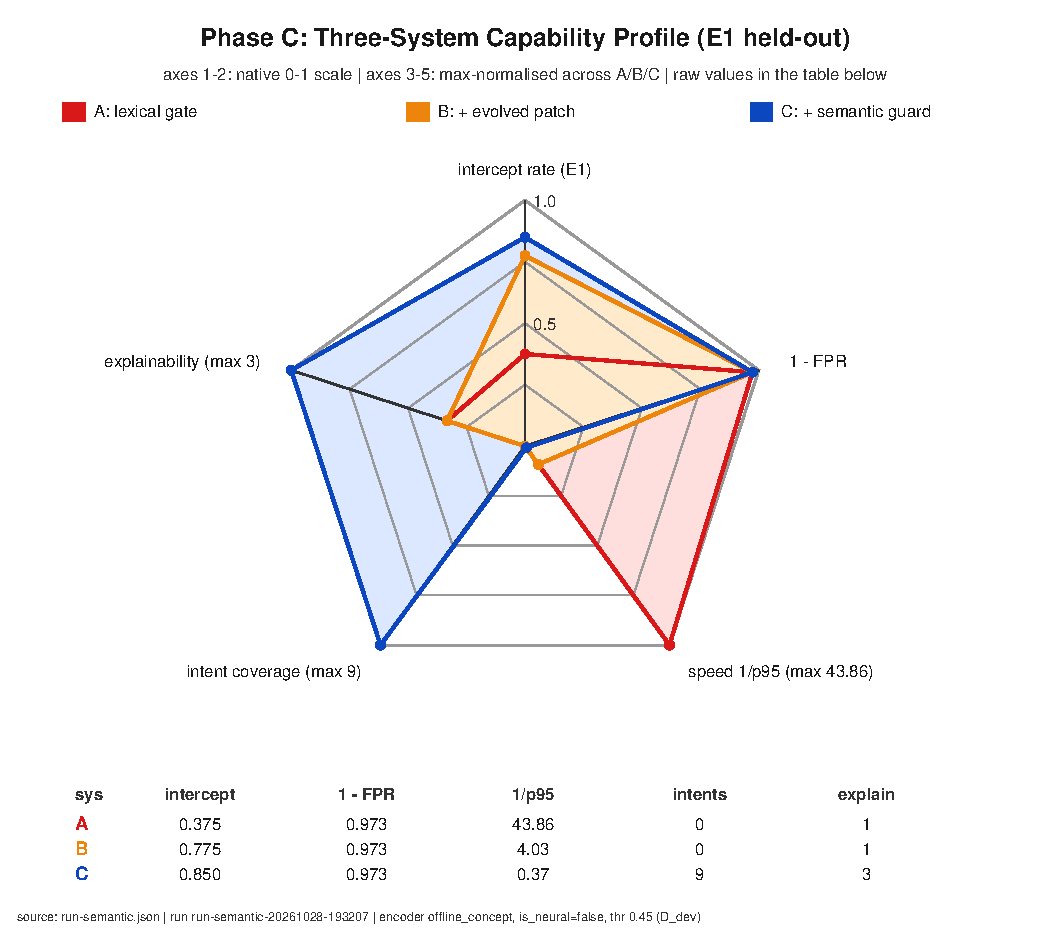
\includegraphics[width=\textwidth]{phase_c_radar.pdf}
\caption{能力剖面（E1 held-out）。实线：A / B / C-offline；虚线：C-neural 消融。
五轴 = 拦截率（E1）/ 1$-$FPR / 速度（1/p95）/ 覆盖意图数 / 可解释性；前两轴原生
0--1，后三轴按所画序列最大值归一化，原始值见图内表格。\textbf{两个后端的关键
对比：} \texttt{offline\_concept}（thr 0.45，语义 p95 1.78 ms / 完整判定 p95
1.2--1.3 ms，E1 0.850）\textbf{vs} neural MiniLM ONNX（thr 0.69，语义 p95
8.49 ms / 完整判定 p95 11.9--14.8 ms，E1 0.775）。神经变体在速度轴上内缩明显，
拦截率也更低；C-hybrid 与 C-offline 拦截率相同、只是更慢，未画（原始值见
\texttt{figure\_data.json}）。来源同图~\ref{fig:supp-comparison}。}
\label{fig:supp-radar}
\end{figure}

\section{复现、验证与诚实边界}

\textbf{复现。}\ 图由 \texttt{tools/plot\_phase\_c.py} 从三份 run JSON +
消融 JSON 生成（缺任何字段即退出码 2 并点名，不手填）；图与全部落图数值在
\texttt{experiments/phase-c/figures/}。本补充材料由 XeLaTeX 从
\texttt{paper/supplementary-phase-c.tex} 编译，命令见文件头注释。

\textbf{诚实边界。}
\begin{itemize}
  \item $E_1$/$E_0$ 是 held-out 变体、不是 OOD；$E_0$ 只是新随机实现。
  \item 样本量：每组 40 条；$D_{\mathrm{dev}}$ 穿透样本 111 条；结论是"证据
    支持/指示"，不是"证明"。
  \item 延迟是单机 CPU 实测（无并发、无网络）；神经变体含 ONNX int8 推理，
    冷启动离群点 1.0 s 为单条记录；两种延迟口径不得混用。
  \item M/R/B 标签是评估方预注册判定，消除事后拟合但保留人工判断。
  \item 良性语料 74 条不含俄/阿文本，跨语种误伤对两个编码器都未被样本检验。
  \item 神经模型是 ONNX int8 的 CPU 导出，其延迟不能当作原始框架模型的延迟。
  \item 概念编码器仍无法处理完全无共享词法证据的改写；残余漏拦见
    \texttt{residual\_misses\_C}。
\end{itemize}

\end{document}
